\chapter{Background Theory}
\label{ch:background}

\section{Edit difference algorithms}
To measure difference between different text revisions, we will refer
edit distance. Edit distance between two texts, as first defined by
Levenshtein,\cite{Levenshtein1966} can be defined as the minimum
amount of insert, delete and substitutions operations needed to
transform one text into another. We find a trivial illustration of
this in figure~\ref{fig:fork-spork}

\begin{figure}
  \centering
  
  \begin{tikzpicture}[node distance =3pt and 0.5cm,anchor=center]
    
    \matrix[table] (mat11) { |[fill=greeni]| &
      |[fill=yellowi]|F & O & R & K & |[fill=redi]|S
      \\ |[fill=greeni]|S & |[fill=yellowi]|P & O & R & K &
      |[fill=redi]| \\ };

    \CellText{11-1-1}{string 1:}; \CellText{11-2-1}{string
      2:};

    \SlText{11-1-1}{Insert} \SlText{11-1-2}{Swap}
    \SlText{11-1-6}{Delete}
    
  \end{tikzpicture}

  \vspace{3 mm}

  forks $\rightarrow$ spork, edit distance: 3
  
  \caption{An edit distance example using all three basic edit
    operations}
  \label{fig:fork-spork}
\end{figure}

\begin{figure}
  \label{fig:levdef}
  \centering
  for the function $\mbox{lev}_{a,b}(|a|,|b|)$:\\
  $$\mbox{lev}_{a,b}(i,j) = 
  \left\{
  \begin{array}{ll}
    \mbox{max}(i,j) & \mbox{if }min(i,j) = 0\\
    \mbox{min}\left\{
    \begin{array}{lll}
      lev_{a,b}(i-1,j)+1\\
      lev_{a,b}(i,j-1)+1\\
      lev_{a,b}(i-1,j-1)+1_{(a_i{\neq}b_j)}
    \end{array}
    \right.
    & else 
  \end{array}
  \right.$$
  when $a_i = b_j$, $1_{(a_i{\neq}b_j)} = 1$\\
  when  $a_i \neq b_j$, $1_{(a_i{\neq}b_j)} = 0$
  \caption{The definition of Levenshtein edit distance.}
\end{figure}

Levenshtein's characterisation of this distance is given in
figure~\ref{fig:levdef}. It defines that the distance between two
strings is characterised the minimum distance between three different
pair-combinations of its substrings. A 'text-book' implementation of
this algorithm can be represented by the pseudo-code below. (We
present the dynamic-programming-style algorithm here, and will
generally be working with dynamic programming implementations
throughout the study.)

\begin{figure}
  \centering
  \begin{lstlisting}
    ed(x,y):
    #end base cases
    if |x| = 0: return |y|
    if |y| = 0: return |x|    

    #end table initialisation
    d is a table [0..|x|][0..|y|]
    for i = 1 to |m|:
    d[i,0] = i
    for j = 0 to |y|:
    d[0,j] = j           
    
    #dynamic computation
    for j = 1 to |y|:
    for i = 1 to |x|:
    c = [(x[i] == y[j]) ? O else 1]
    ins = d[i-1,j] + 1
    dlt =d[i,j-1] + 1
    kp_swp = d[i-1,j-1] + c
    d[i,j] = min(ins, dlt, kp-swp)
    
    #return last computed number
    return d[|x|,|y|]
  \end{lstlisting}
  \caption{Basic dynamic implementation of Levenshtein distance}
  \label{fig:levenshtein-dynamic}
\end{figure}

In figure~\ref{levenshtein-dynami} we find a dynamic programming
implementation of Levenshtein - the basic 'textbook'
implementation. We can see that on comparing strings $x$ and $y$, a
$|x|$ by $|y|$ table is created, and then filled with values. For this
reason both the time and space complexity of the algorithm is $\theta
(|x||y|)$.

Reducing the space needed for this computation is relatively easy, and
can be done in a few different ways. One way is to simply disregard
parts of the table already computed. We can see that, on each
computation of $d[i,j]$ (as it appears above), we require only a small
part of the matrix: $d[i-1,j-1]$, $d[i-1,j]$ and $d[i,j-1]$. At any
iteration $i$, where is great than $1$, we may disregard rows $0 \dots
(i-2)$ inclusive.

There are more complicated techniques that allow us to also disregard
unneccesary computation --- a few implementations employ strategies
that allow them to trace the table space diagonally, rather than
iteratively, achieving a time complexities as low as $O(ed(x,
y)^2)$.\cite{Chang1992} Another harnesses bit vectors to achieve a
time complexity of $O(nm/w)$ or $O(nm log {\Sigma}/w)$ time where $w$
the bit-word size of the machine, and $\Sigma$ is the alphabet
size.\cite{Myers1999}\cite{Hyyro2003} 

In this project, however, it was suffice to simply reduce the space
needed for the computation. The texts were relatively small, and the
program was sped up using some simple threading operations. We talk
more about our implementation of edit distance later in the report. 

\subsection*{Varieties of edit distance}
Modifications can be made to the nature of the distance itself, in
order to adapt the measure a variety of different and specific
needs. Here is a brief overview of the main groups these extensions
fall into:

\begin{itemize}
\item \textbf{Hamming distance.} This allows for substitutions only,
  comparing same-length strings, such
  that:\\ $ed_{hamming}(\text{``abc''},\text{``abd''})
  =1$,\\ $ed_{hamming}(\text{``abc''},\text{``bcd''}) = 3$,\\ and
  $ed_{hamming}(\text{``abc''},\text{``ab''})$ is
  undefined.\cite{Hamming1950}
\item \textbf{Reversals.} The Damerau-Levenshtein distance defines an
  `swap' operation, which is the reversal of two adjacent
  characters. It is particularly suited to spell-checking, and for
  analysing DNA-sequence variations. In this
  case:\\ $ed_{damerau}(\text{``ab''},\text{``ba''}) = 1$
\item \textbf{Block distance.} This allows for displacements of entire
  blocks to count as one operation. For
  example:\\ $ed_{block}(\text{``abcde''},\text{``cdeax''})= 2$ \\ One
  move of the block `cde', one substitution of `b' for
  `x'.\cite{Tichy1984}
\item \textbf{\textit{q}-grams distance.} \textit{q}-grams are simply
  sub-strings, and this measure describes the similarity of two
  strings in terms of \textit{q}-grams they
  share.\cite{Ukkonen1992}\\ $ed_{q-gram}(x,y)=\sum\limits_{v\in\Sigma
    ^q}|G(x)[v]-G(y)[v]|$\\ where $G(x)[v]$ returns the number of
  occurrences of \textit{q}-gram v in string x, and $\Sigma ^q$ is all
  the possible \textit{q}-grams in the alphabet (capped by string
  length). $|G(x)[v]-G(y)[v]|$ a large positive number every time a
  \textit{q}-gram appears a large amount of times in one string, but
  not the other; it returns 0 if the substring apears the same number
  of times. So, the whole function measures this difference for all
  possible substrings, and sums them, returning a high number for
  difference, and a low number for similarity.
\end{itemize}

Other algorithms we may look at are those that, like the
\textit{q}-gram distance, principally concern themselves with finding
common subsequences between the strings. The common subsequence
problem relates to the editdistance problem by way of the
heuristic that two similar strings will have similar subsequences ---
the \textit{q}-gram algorithm, for instance, relies on this heuristic,
and works well for most texts, it does not agree with all distance
measures. For example, two strings that are very different according
to this heuristic may be quite similar according to the
Damrau-Levenshtein measure.

\subsection*{Optimal alignment}
Another part of the problem of working out optimal edit distance is
finding the `optimal alignment' --- the measures are closely
related. We displace and arrange the characters of a string such that
the set of operations to transform each character into its counterpart
is minimal. For example, in figure \ref{fig:fork-spork}, the alignment
of the two strings ``fork'' and ``spork'' was:

\begin{center}
  \begin{tabular}{cccccc}
    s & p & o & r & k & -\\
    - & f & o & r & k & s 
  \end{tabular}
\end{center}

However it could also conceivably have been:

\begin{center}
  \begin{tabular}{ccccccccccccccccc}
    s & p & o & r & k & - & & or even & & - & s & p & o & - & r & k &\\
    f & - & o & r & k & s & &         & & f & - & o & - & r & k & - & s    
  \end{tabular}
\end{center}

Here, the left-hand version results in an equivalent
Levenshtein distance, but we can see how the distance for the
right-hand example would be sub-optimal.

\begin{figure}[h]
  \centering   
  \begin{tikzpicture}[node distance =3pt and 0.5cm,anchor=center]
    \matrix[table] (mat11) {|[fill=greeni]|  & |[fill=redi]|S & |[fill=yellowi]|P & |[fill=redi]|O & |[fill=greeni]|  & |[fill=redi]|R & K & |[fill=greeni]|\\
      |[fill=greeni]|F & |[fill=redi]|  & |[fill=yellowi]|O & |[fill=redi]|  & |[fill=greeni]|R & |[fill=redi]|  & K & |[fill=greeni]|S\\};
    
    \CellText{11-1-1}{string 1:}; \CellText{11-2-1}{string
      2:};

    \SlText{11-1-1}{Insert}
    \SlText{11-1-2}{Delete}
    \SlText{11-1-3}{Swap}
    \SlText{11-1-4}{Delete}
    \SlText{11-1-5}{Insert}
    \SlText{11-1-6}{Delete}
    \SlText{11-1-8}{Insert}
  \end{tikzpicture}\\
  \vspace{3 mm}
  spork $\rightarrow$ forks, edit distance: 7
  \caption{An sub-optimal edit distance example}
  \label{fig:fork-spork-subopt}
\end{figure}

The Smith-Waterman algorithm calculates optimal alignment by
populating two tables --- one like that in the pseudocode
above, and also as a table of arrows. These arrows define a
path from one corner of the table space to the other. The
shape of this path defines how to align the two
strings.\cite{Smith1981} See figure
\ref{fig:smith-waterman-traceback} for an example.

This path may also be read as an edit operation. An arrow at the
position $[i,j]$ in the table defines edit operations for $x[i]$
and/or $y[j]$ thus:
\begin{itemize}
\item \textbf{$\nwarrow$ at $[i,j]$, if $x[i] \neq y[j]$} \\ Denotes a
  'swap' between $x[i]$ and $y[j]$ (if $x[i] = y[j]$ then it denotes
  the lack of an operation).
\item \textbf{$\uparrow$ at $[i,j]$}\\Denotes the deletion of $x[i]$
\item \textbf{$\leftarrow$ at $[i,j]$}\\Denotes the insertion of
  $y[j]$
\end{itemize}

\begin{figure}[h]
  \centering $\left\{
  \begin{array}{ccccccc}
    & & S & P & O & R & K \\ & \color{red}{0} & \color{red}{0} & 0 & 0
    & 0 & 0 \\ F & 0 & \nwarrow & \color{red}{\nwarrow} & \nwarrow &
    \nwarrow & \nwarrow \\ O & 0 & \uparrow & \nwarrow &
    \color{red}{\nwarrow} & \downarrow & \leftarrow \\ R & 0 &
    \uparrow & \uparrow & \uparrow & \color{red}{\nwarrow} &
    \leftarrow \\ K & 0 & \uparrow & \uparrow & \uparrow & \uparrow &
    \color{red}{\nwarrow} \\ S & 0 & \nwarrow & \uparrow & \uparrow &
    \uparrow & \color{red}{\uparrow} \\
  \end{array}\right\} $\\
  (If the arrow reaches an edge before the left-hand corner, we trace
  along that edge, reading each shift as an arrow in the direction of
  the trace.)
  \caption{Diagram showing Smith-Waterman traceback path (in red) on
    the edit operation forks $\rightarrow$ spork}
  \label{fig:smith-waterman-traceback}
\end{figure}

\subsection*{Delta encoding}
Finally, we may also look into Delta encoding algorithms. These
describe ways of compressing the storage of a document's history --- a
format in which only the differences between each text is stored, not
the entire version. These algorithms are of the same family of
algorithms discussed above. In fact, we find that one of the fastest
known algorithms,\footnote{According to Hunt's 1998
  study\cite{Hunt1998}} \textit{VDelta}, is a refinement of the block
distance algorithm mentioned above. For a given version $n$ of a
document $doc$ is defined as:

$$v_n = v_0 \cup {\Delta}(v_0,v_1) \cup {\Delta}(v_1,v_2) \cup \dots
\cup {\Delta}(v_{n-1},v_n) $$

where ${\Delta}(v_i,v_j)$ is the difference between version $i$ and
version $j$ of the document, and the union operation $\cup$ combines
each version in a manner particular to the $\Delta$ data-type. Storing
data in this way can be very efficient, resulting in a compression
factors of five or ten on typical data.\cite{Macdonald2000} It may
also be relatively easy to maintain in our case, due to the linear
nature of Wikipedia revision histories.

%%%%%%%%%%%%%%%%%%%%%%%%%%%%%%%%%%%%%%%%%%%%%%%%%%%%%%%%%%%%
%%
%% WIKIPEDIA
%%
%%%%%%%%%%%%%%%%%%%%%%%%%%%%%%%%%%%%%%%%%%%%%%%%%%%%%%%%%%%%
\section{Wikipedia}
\subsection*{In academia}
Wikipedia is a free, open-source, publicly-editable online
knowledge-base. The software is runs upon, PHP-based MediaWiki, is
also open-source, powering countless other online encyclopedias. The
website is ranked 6\super{th} globally in terms of website traffic,
and is the highest-ranked reference website by far - most of the sites
it shares the top spots with are portals, search engines, shopping
mega-sites, and social media websites.\footnote{According to `Alexa',
  an website ranking company.\cite{Alexa-about2014} Though, this may
  be an underestimation. Alexa may well be biased towards English
  speakers and Internet Explorer users, underestimating
  Wikipedia.org's popularity, since `two thirds of all Wikipedia
  articles are in languages other than
  English'\cite{wikimedia-noteonalexa}} Despite early skepticism
(particularly concern over the inherent chaos in the system:
``...edits, contributed in a predominantly undirected and haphazard
fashion by ... unvetted volunteers.''\cite{Wilkinson2007}), it is
widely claimed to be a success, `the best-developed attempt thus far
of the enduring quest to gather all human knowledge in one
place'\cite{Mesgari2014}.

That Wikipedia has become a hub of research in many fields is also
self-evident to anyone who has searched for articles on the
subject. Mesgari et al, just quoted, has prepared a very recent
`systematic review of scholarly research on the content of Wikipedia',
which gives an overview of 110 articles on the subject --- attesting
to his observation that Wikipedia has been `irresistable point of
unquiry for researchers from various fields of knowledge'. It will be
a useful touching stone for this study, finding 82 out of the 110
surveyed articles to concern Wikipedia quality. Some of these are also
referenced here, and many of the others will come to bear on the study
as it progresses.

Other important general sources will be WikiLit,\cite{wikilit}
AcaWiki\cite{acawiki} and WikiPapers\cite{wikipapers}, all of which
are online repositories of academic research into Wikipedia and other
Wikis.

%%%%%%%%%%%%%%%%%%%%%%%%%%%%%%%%%%%%%%%%%%%%%%%%%%%%%%%%%%%%
%%
%% WIKIPEDIA ARTICLE QUALITY
%%
%%%%%%%%%%%%%%%%%%%%%%%%%%%%%%%%%%%%%%%%%%%%%%%%%%%%%%%%%%%%

\subsection*{Studies of Wikipedia revision history}
Tangentialy related studies fall into two major groups: studies of
Wikipedia article quality and studies of edit behaviour.  It is from
the first group that we find the most pertinent work --- it is also
one of the most fruitful areas of research.

It is the metrics used to measure quality in these studies that are of
most use to us here. We don't concern ourselves with the quality of
the article on the whole, but many studies have endeavoured to find
out what kind of article content can be automatically recognised. High
numbers of Links, internal links, images and formulas have been found
to indicate percieved quality,\cite{Lucassen2010}\cite{mcguinness2006}
and these are easy to identify using Wikipedia's markup
language. Other useful meterics have been the age of the
word,\cite{Cross2006} the age and rate of change of the article in
comparison to other articles,\cite{Zeng2006} and the recent activity
of the article (an article undergoing a peak in edit changes may be
`unstable').\cite{Adler2006} Another study of particular interest is
that of Stvilia et al, which found metrics of article quality through
factor analysis,\cite{Stvilia2005} confirming much of the ideas
already mentioned.

A landmark piece of work is the Wikitrust software.\cite{Adler2007}
Wikitrust was\footnote{Defunct as of author's checks, Apr 2014} a
firefox plugin, designed to highlight the words of a Wikipedia article
with different colors. The gradations of these colors relate to levels
of trust, and the computations made to derive them were based upon the
metrics mentioned above, with particular emphasis on a word's age. A
screenshot can be seen in figure \ref{fig:wikitrust}. The program was
reviewed as recently as 2011,\cite{Lucassen2011} and it was found to
be basically flawed, with users not really seeing the use for it (it
was found that, having read Wikipedia before, they already had a good
idea of how to rate an article). However, the Wikitrust team's
implementation of the quality measures described above will prove to
be very useful study.

\begin{figure}
  \centering
  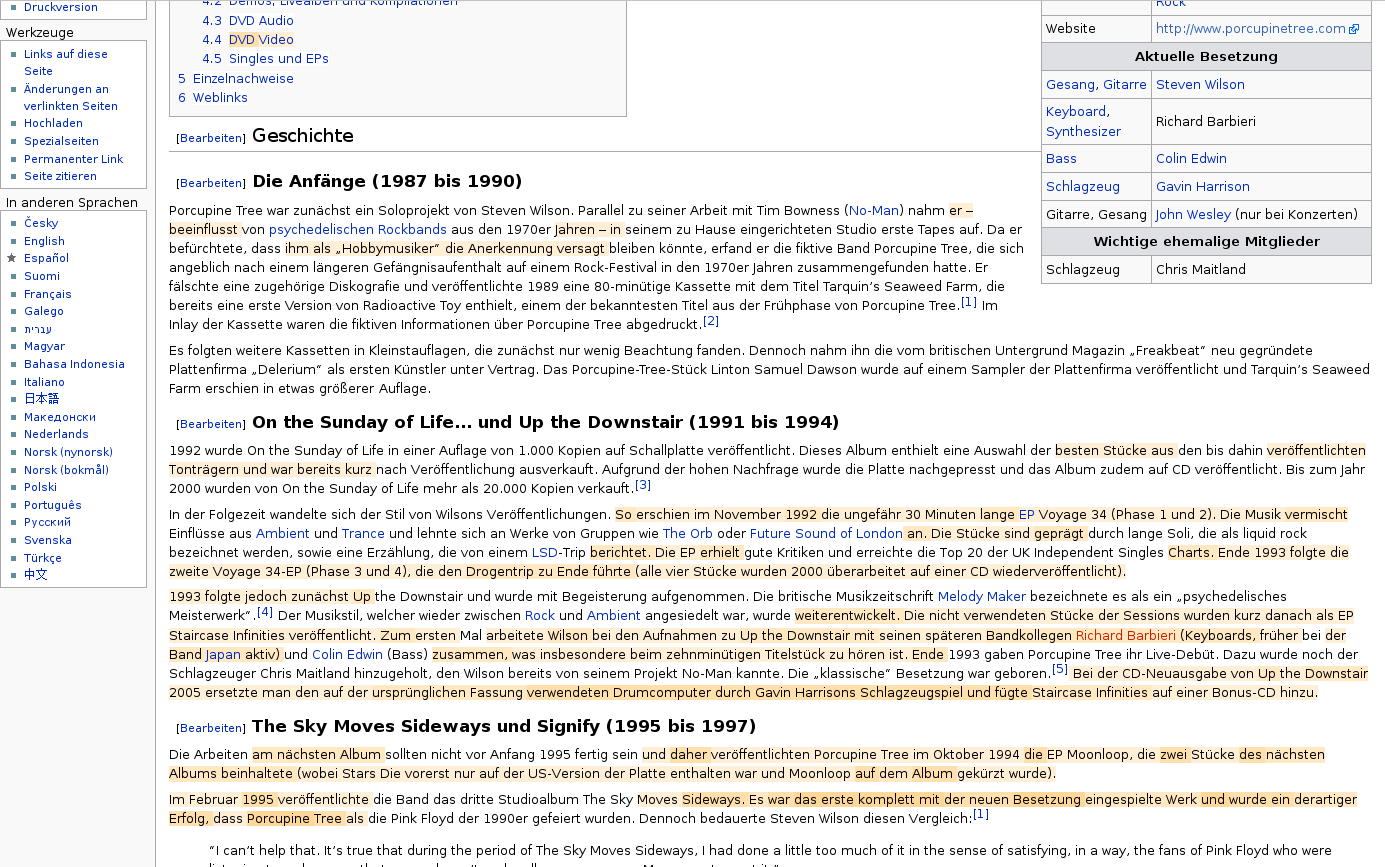
\includegraphics[width=0.8\textwidth,clip=true,resolution=300]{img/wikitrust.png}
  \caption{Wikitrust in action, 2011}
  \label{fig:wikitrust}
\end{figure}

Another metric which may also affect the quality of an article as a
resource, is logical structure. It was found in 2005 that this, if
anything, was the clearest difference between Wikipedia and commercial
encyclopedias,\cite{Giles2005} supporting previous
conjecture.\cite{Denning2005} Not many studies have concerned
themselves with structure, but later we will discuss how we may
automatically recognise structural change.

A few other key studies present us with useful analyses of edit
behaviour. Analyses of conflict between authors shows the possible
reversion cases we will have to recognise. They reveal the high number
of immediate `undo'-type revisions, and also that malicious or
unnecessary input may survive several versions before being
undone. Some study these conflicts as a characterisation of normal
editing
behaviour,\cite{Kittur2007}\cite{Kittur2009}\cite{Kittur2010}\cite{Potthast2008}
while others look to controversial articles,\cite{Iba2010} or articles
recently cited in the press.\cite{Lih2004} We find from these same
studies that articles lead by small groups of `leaders' produce
articles of better quality than those with a more homogeneous
contribution group, that a small group of editors contribute to most
of Wikipedia, and that conflict and bureaucracy (increasing over time)
are the major limiting factors in the growth of an
article.\cite{Suh2009} Knowledge of this context is vital in
evaluating the edits we will eventually analyse.
